\documentclass[12pt]{article}

\usepackage{graphicx}
\usepackage{paralist}
\usepackage{amsfonts}
\usepackage{amsmath}
\usepackage{hhline}
\usepackage{booktabs}
\usepackage{multirow}
\usepackage{multicol}
\usepackage{url}
\usepackage{listings}

\oddsidemargin -10mm
\evensidemargin -10mm
\textwidth 160mm
\textheight 200mm
\renewcommand\baselinestretch{1.0}

\pagestyle {plain}
\pagenumbering{arabic}

\newcounter{stepnum}

%% Comments

\usepackage{color}

\newif\ifcomments\commentstrue

\ifcomments
\newcommand{\authornote}[3]{\textcolor{#1}{[#3 ---#2]}}
\newcommand{\todo}[1]{\textcolor{red}{[TODO: #1]}}
\else
\newcommand{\authornote}[3]{}
\newcommand{\todo}[1]{}
\fi

\newcommand{\wss}[1]{\authornote{blue}{SS}{#1}}

\title{Assignment 4, Design Specification}
\author{SFWRENG 2AA4}

\begin{document}

\maketitle
This Module Interface Specification (MIS) document contains modules, types and
methods for implementing the game \textit{2048}. A game commences by initializing a game board with two of the 16 tiles in the board populated by either a 2 or a 4. The user can choose whether they would like to move up by entering the number 1, move down by entering the number 2, move left by entering the number 3, or move right by entering the number 4. All of the tiles in the gameboard will shift according to the user's move. If two tiles that have the same value are moved in the appropriate direction, the two tiles will combine to form one tile, where its value will be the added value of the two equal tiles. The game can terminate in three ways. If the user wishes to exit the game, the number 0 can be entered. If there are no possible moves that the user can make to change the state of the gameboard, then the game terminates and the user has lost. If one of the tiles has a value of 2048, the game terminates and the user has won. The game can be launched and played by typing \texttt{make play} in terminal.

\begin{center}
  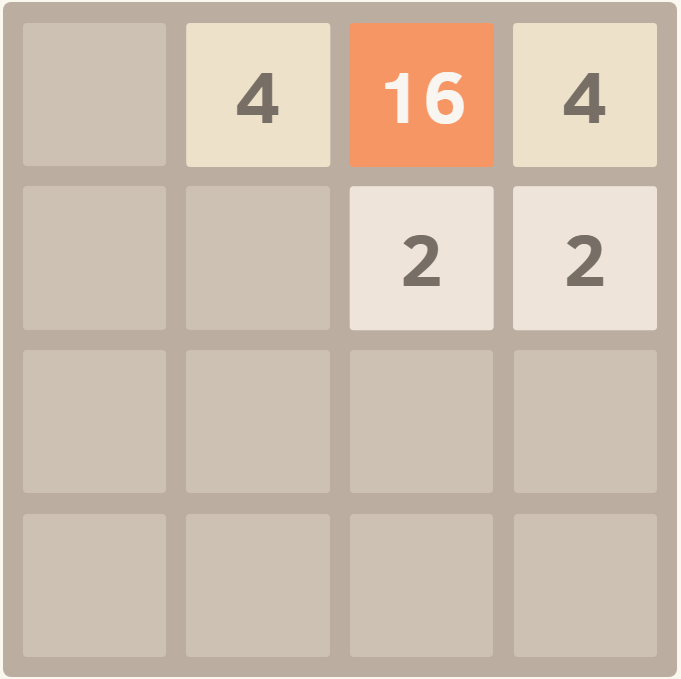
\includegraphics[width=0.4\textwidth]{2048.png}

  The above board is from https://play2048.co/
\end{center}

\newpage

\section{Overview of the design}

The implemented design successfully applies the Module View Specification design pattern and applies the Module View Specification (MVC) design pattern. The MVC components
are \textit{MoveController} (controller module), \textit{BoardT} (model module), and \textit{Display} (view module). In addition to the MVC design pattern, a library module is used that encompasses static functions that are used by the model module for certain methods. A main function, \textit{Play.java} allows for the game to be run with all three modules using one another as intended. 

\bigskip

\noindent The UML diagram below provides a visualization of the structure of the designed software architecture.

\begin{center}
  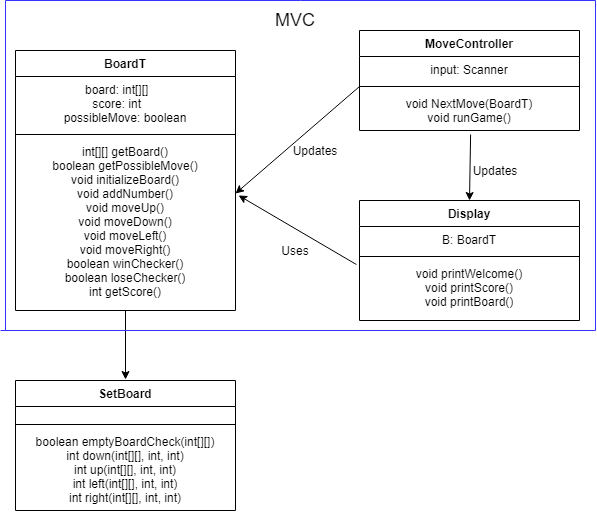
\includegraphics[width=0.6\textwidth]{UMLA4.png}
\end{center}

\bigskip

The model module \textit{BoardT}
stores the state of the game board as well as its status. The view module \textit{Display} represents the game board visually through the terminal using text-based graphics. Finally, the controller \textit{MoveController} is responsible for handling input actions. The MVC design pattern is specified and implemented in a way such that the display and controller use an instance of BoardT, and the controller effecitvely updates the contents of the display based on the user's input. The user is given the choice to execute their next move, or exit from the game based on the properties of the \textit{MoveController}. Additionally, specific methods of the \textit{BoardT} determine whether the game is in a winning or losing state, in which the game is terminated as well. 

\newpage

\subsection*{Likely Changes my design considers:}

\begin{itemize}
  \item The visual representation of the game such as a graphical user interface layout. 
  \item Change in game modes by increasing/decreasing the dimensions of the board, or increased difficulty through different winning conditions
  \item Change in scanner for taking user input such as using a KeyListener
  \item Data structure used for storing the board
  \item Change variable type for inputted board



\end{itemize}


\newpage

\section* {SetBoard Module}

\subsection*{Template Module}

SetBoard

\subsection* {Uses}

None

\subsection* {Syntax}

\subsubsection* {Exported Constants}

None

\subsubsection* {Exported Types}

None

\subsubsection* {Exported Access Programs}

\begin{tabular}{| l | p{6cm} | l | p{2.5cm} |}
  \hline
  \textbf{name} & \textbf{In} & \textbf{Out} & \textbf{Exceptions}\\
  \hline
  emptyBoardCheck & seq of (seq of $\mathbb{N})$ & $\mathbb{B}$ & \\
  \hline
  down & seq of (seq of $\mathbb{N})$, $\mathbb{N}$, $\mathbb{N}$ & $\mathbb{N}$ & \\
  \hline
  up & seq of (seq of $\mathbb{N})$, $\mathbb{N}$, $\mathbb{N}$ & $\mathbb{N}$ & \\
  \hline
  left & seq of (seq of $\mathbb{N})$, $\mathbb{N}$, $\mathbb{N}$ & $\mathbb{N}$ & \\
  \hline
  right & seq of (seq of $\mathbb{N})$, $\mathbb{N}$, $\mathbb{N}$ & $\mathbb{N}$ & \\
  \hline
\end{tabular}

\subsection* {Semantics}

\subsubsection* {State Variables}

None

\subsubsection* {State Invariant}

None

\subsubsection* {Assumptions}
\begin{itemize}
  \item Complete access to the Random java utility library is available
\end{itemize}

\subsubsection* {Access Routine Semantics}

\noindent emptyBoardCheck(board):
\begin{itemize}
\item output: $out$ := (Arrays.deepEquals(emptyBoard, board) $\Rightarrow$  true $|$ $\text{True}$ $\Rightarrow$ false)
\newline where $\mathit{emptyBoard} \equiv$ [[0, 0, 0, 0], [0, 0, 0, 0], [0, 0, 0, 0], [0, 0, 0, 0]]
\item exception: none
\end{itemize}

\noindent down(board, row, col):
\begin{itemize}
\item output: $out$ := (row $<$ 3 $\Rightarrow$  board[row+1][col] $|$ $\text{True}$ $\Rightarrow$ 1)
\item exception: none
\end{itemize}

\noindent up(board, row, col):
\begin{itemize}
\item output: $out$ := (row $>$ 0 $\Rightarrow$  board[row-1][col] $|$ $\text{True}$ $\Rightarrow$ 1)
\item exception: none
\end{itemize}

\noindent left(board, row, col):
\begin{itemize}
\item output: $out$ := (col $>$ 0 $\Rightarrow$  board[row][col-1] $|$ $\text{True}$ $\Rightarrow$ 1)
\item exception: none
\end{itemize}

\noindent right(board, row, col):
\begin{itemize}
\item output: $out$ := (col $<$ 3 $\Rightarrow$  board[row][col+1] $|$ $\text{True}$ $\Rightarrow$ 1)
\item exception: none
\end{itemize}

\subsubsection* {Local Functions}

Arrays.deepEquals: seq of (seq of $\mathbb{N}) \times$ seq of (seq of $\mathbb{N}) \rightarrow \mathbb{B}$ 

\medskip

\noindent Array.deepEquals($a, b$) $\equiv$ $(\forall x \cdot (\forall y \cdot a_{xy} = b_{xy}))$ 


\newpage

\section* {Board ADT Module}

\subsection*{Template Module}

BoardT

\subsection* {Uses}

SetBoard

\subsection* {Syntax}

\subsubsection* {Exported Types}

None

\subsubsection* {Exported Constant}

SIZE = 4 \quad // Size of the board which is assumed to always be 4 x 4

\subsubsection* {Exported Access Programs}

\begin{tabular}{| l | l | l | l |}
\hline
\textbf{Routine name} & \textbf{In} & \textbf{Out} & \textbf{Exceptions}\\
\hline
BoardT & seq of (seq of $\mathbb{N}$) & BoardT & \\
\hline
getBoard & ~ & seq of (seq of $\mathbb{N}$) & \\
\hline
getPossibleMove & ~ & seq of (seq of $\mathbb{B}$) & \\
\hline
initializeBoard & ~ & $ ~ $ & \\
\hline
addNumber & ~ & $ ~ $ & \\
\hline
moveUp & ~ & $ ~ $ & \\
\hline
moveDown & ~ & $ ~ $ & \\
\hline
moveLeft & ~ & $ ~ $ & \\
\hline
moveRight & ~ & $ ~ $ & \\
\hline
winChecker & ~ & $ \mathbb{B} $ & \\
\hline
loseChecker & ~ & $ \mathbb{B} $ & \\
\hline
getScore & ~ & $ \mathbb{N} $ & \\
\hline
\end{tabular}

\subsection* {Semantics}

\subsubsection* {State Variables}

board: sequence [Size, Size] of $\mathbb{N}$ \\
score: $\mathbb{N}$ \\
possibleMove: $\mathbb{B}$

\subsubsection* {State Invariant}

None

\subsubsection* {Assumptions}

\begin{itemize}
  \item The constructor BoardT is called for each object instance before any other access routine 
  is called for that object. 
  \item Assume there is a random function that generates a random value beteern 0 and 1.
  \item Complete access to the Random java utility library is available
  \item The addNumber method will always be called following a possible move
\end{itemize}

\subsubsection* {Access Routine Semantics}

\noindent BoardT($board$):
\begin{itemize}
\item transition: board, score, possibleMove $=$ $board$, 0, $false$
\item output: $out := \mathit{self}$
\item exception: None
\end{itemize}

\noindent getBoard():
\begin{itemize}
\item transition: none
\item output: $out :=$ board
\item exception: None
\end{itemize}

\newpage

\noindent getPossibleMove():
\begin{itemize}
\item transition: none
\item output: $out :=$ possibleMove
\item exception: None
\end{itemize}

\noindent InitializeBoard():
\begin{itemize}
\item transition: 
\begin{lstlisting}
if(SetBoard.emptyBoardCheck(this.board)) {
	addNumber();
	addNumber();
}
\end{lstlisting}
\end{itemize}

\noindent addNumber():
\begin{itemize}
\item transition: 
\begin{lstlisting}
	String numstring = "4222222222"
	for(int i = 0; i < SIZE; i++) {
            for(int j = 0; j < SIZE; j++) {
                if(this.board[i][j] == 0) {
                    count++;
                }
            }
        }
        String[] storeFreeBlocks = new String[count];
        int localcounter = 0;
        for(int i = 0; i < SIZE; i++) {
            for(int j = 0; j < SIZE; j++) {
                if(this.board[i][j] == 0) {
                    storeFreeBlocks[localcounter] = "i, j";
                    localcounter++;
                }
            }
        }
        int[] getRowCol = storeFreeBlocks[randomNum]
        int a = getRowCol[0];
        int b = getRowCol[1];
        this.board[a][b] = Integer.parseInt(numstring);
\end{lstlisting}
\end{itemize}

\noindent moveUp():
\begin{itemize}
\item transition: All values within $this.board$ that are not zero must be shifted upwards if there is a zero above it. If the number directly above the selected cell is equal to the selected cell itself, and is not equal to zero, the cell above becomes double this amount, and the cell below becomes zero. Once any necessary combines have occured, a second shit of the cells upwards must be done to clean up the board following the combine.
\end{itemize}

\noindent moveDown():
\begin{itemize}
\item transition: All values within $this.board$ that are not zero must be shifted downwards if there is a zero below it. If the number directly below the selected cell is equal to the selected cell itself, and is not equal to zero, the cell below becomes double this amount, and the cell above becomes zero. Once any necessary combines have occured, a second shit of the cells downwards must be done to clean up the board following the combine.
\end{itemize}

\noindent moveLeft():
\begin{itemize}
\item transition: All values within $this.board$ that are not zero must be shifted leftwards if there is a zero to the left of it. If the number directly to the left of the selected cell is equal to the selected cell itself, and is not equal to zero, the cell to the left becomes double this amount, and the cell to the right becomes zero. Once any necessary combines have occured, a second shit of the cells leftwards must be done to clean up the board following the combine.
\end{itemize}

\noindent moveRight():
\begin{itemize}
\item transition: All values within $this.board$ that are not zero must be shifted rightwards if there is a zero to the right of it. If the number directly to the right of the selected cell is equal to the selected cell itself, and is not equal to zero, the cell to the right becomes double this amount, and the cell to the left becomes zero. Once any necessary combines have occured, a second shit of the cells rightwards must be done to clean up the board following the combine.
\end{itemize}

\noindent winChecker():
\begin{itemize}
\item transition: none
\item output: $out :=$ $(\forall x \cdot (\forall y \cdot (board_{xy} =$ 2048) $\Rightarrow$ true $|$ $\text{True}$ $\Rightarrow$ false))
\item exception: None
\end{itemize}

\noindent loseChecker():
\begin{itemize}
\item transition: none
\item output: $out :=$ 
\begin{lstlisting}
        for(int i = 0; i < SIZE; i++) {
            for(int j = 0; j < SIZE; j++) {
                if(this.board[i][j] == 0) {
                    return false;
                }
                if (i > 0 && this.board[i-1][j] == this.board[i][j]) {
                  return false;
                }
                if (i < SIZE-1 && this.board[i+1][j] == this.board[i][j]) {
                  return false;
                }

                if (j > 0 && this.board[i][j-1] == this.board[i][j]) {
                  return false;
                }

                if (j < SIZE-1 && this.board[i][j+1] == this.board[i][j]) {
                  return false;
                }
            }
        }
        return true;
    }
\end{lstlisting}

\item exception: None
\end{itemize}

\noindent getScore():
\begin{itemize}
\item transition: none
\item output: $out :=$ score
\item exception: None
\end{itemize}

\newpage

\section* {Display Module}

\subsection* {Display Module}

\subsection* {Uses}

BoardT, Move

\subsection* {Syntax}

\subsubsection* {Exported Types}

None

\subsubsection* {Exported Constants}

BOARD = [[0, 0, 0, 0], [0, 0, 0, 0], [0, 0, 0, 0], [0, 0, 0, 0]] 	// Empty Game Board

\subsubsection* {Exported Access Programs}

\begin{tabular}{| l | l | l | p{6cm} |}
\hline
\textbf{Routine name} & \textbf{In} & \textbf{Out} & \textbf{Exceptions}\\
\hline
printWelcome & ~ & ~ & \\
\hline
printScore & ~ & ~ & \\
\hline
printBoard & ~ & ~ & \\
\hline
\end{tabular}

\subsection* {Semantics}

\subsection*{Environment Variables}

window: A portion of the computer screen, specifically the terminal, to display the game and messages.

\subsubsection* {State Variables}

B: BoardT

\subsubsection* {State Invariant}

None

\subsubsection* {Assumptions}

\begin{itemize}
\item The game board used only consists of numbers that are powers of 2.
\item The terminal window is large enough to display the dimensions of the game board, the score, and the prompt for the user's next move
\end{itemize}

\subsubsection* {Access Routine Semantics}

\noindent printWelcome():
\begin{itemize}
\item transition: window $:=$ Displays a welcome message when user first enter the game along with instructions for possible next moves.
\end{itemize}

\noindent printScore():
\begin{itemize}
\item transition: window $:=$ Prints out the updated score after every turn is made
\end{itemize}

\noindent printBoard($board$):
\begin{itemize}
\item transition: window $:=$ Draws the game board onto the screen. The board is first initialized through the $B.initializeBoard$ method if the board is empty. Then the board is formatted using the $B.boardFormatter$ method, so that the user sees a 4x4 grid populated by numbers that are an exponent of 2. The current state of the board is verified to see if the user has lost through the $B.loseChecker$ method, or if the user has won through the $B.winChecker$ method. Then, once the user has inputted their desired next move, the $Move.nextMove$ method will alter the board to reflect the next move made by the user.
\end{itemize}

\newpage

\section* {MoveController Module}

\subsection* {MoveController Module}

\subsection* {Uses}

BoardT, Display

\subsection* {Syntax}

\subsubsection* {Exported Types}

None

\subsubsection* {Exported Constants}

None

\subsubsection* {Exported Access Programs}

\begin{tabular}{| l | l | l | p{4.7cm} |}
\hline
\textbf{Routine name} & \textbf{In} & \textbf{Out} & \textbf{Exceptions}\\
\hline
nextMove & BoardT & & ~ \\
\hline
nextMove & ~ & & ~ \\
\hline
\end{tabular}

\subsection* {Semantics}

\subsection*{Environment Variables}

input: Scanner(System.in) \qquad \textit{// Stores user input representing the desired move.}

\subsubsection* {State Variables}

None

\subsubsection* {State Invariant}

None

\subsubsection* {Assumptions}
\begin{itemize}
\item The user only inputs a number of type $\mathbb{N}$ to reflect their desired turn
\item The user does not wish to immediately play another game once the game baord is deemed to either be in a winning or losing state. The game must be re-run if the game is terminated.
\end{itemize}
\subsubsection* {Access Routine Semantics}

\noindent nextMove($B$):
\begin{itemize}
\item transition: (choice = 0) $\Rightarrow$ System.exit(0); $|$ \newline (choice = 1) $\Rightarrow$ B.moveUp() $\land$ B.getPossibleMove $\Rightarrow$ B.addNumber() $|$ \newline (choice = 2) $\Rightarrow$ B.moveDown() $\land$ B.getPossibleMove $\Rightarrow$ B.addNumber() $|$ \newline (choice = 3) $\Rightarrow$ B.moveLeft() $\land$ B.getPossibleMove $\Rightarrow$ B.addNumber() $|$ \newline (choice = 4) $\Rightarrow$ B.moveRight() $\land$ B.getPossibleMove $\Rightarrow$ B.addNumber() $|$ \newline $\text{True}$ $\Rightarrow$ System.out.println("Move not possible, try again!")
\newline where $\mathit{choice} \equiv$ input.nextInt()
  
\item exception: none
\end{itemize}

\noindent runGame():
\begin{itemize}
  \item transition: operational method for running the game. The game will start with a welcome message as well as explanations surrounding the rules. Every turn, the score and board are printed and updated based on the user's turn.
  \item output: None
\end{itemize}

\subsubsection*{Local Function:}

nextInt: void $\rightarrow$ $\mathbb{Q}$ \\
nextInt() $\equiv$ The user input stored as type integer.

\newpage

\section*{Critique of Design}

\begin{itemize}
  \item The BoardT module, representing the model, is implemented as an abstract data type over an abstract object, because It is more convenient to create a new instance of the board after the user chooses to restart the game. Additionally, the state of the score can be saved and added to following every move through the state variable $this.score$.
  \item By defining the BoardT constructor with a single argument that takes in a 2D array of integers that represents the starting state of the gameboard, the model can be initialized with an empty game board, or any desired game board state for testing purposes.
  \item Essentiality was upheld as a crucial characteristic of the design, as a majority of the functions play a necessary role for creating and updating the game. The display uses print statements, instead of defining void methods that print out these statements to avoid implementing functions that have an output that doesn't change regardless of how the function is called. These print statements are not necessarily required for the implementation of the game, however they were kept in to improve the quality of the view module.
  \item Minimality was upheld by ensuring that all access routines, especially within the Model module, are not independent of one another. Any methods that may have went against the minimality requirement were included as a static method in $SetBoard.java$.
  \item Generality was sacrificed in order to fit the requirements of the game. The modules should perform exactly how the 2048 game performs, and for this reason there is no reason to keep generality in mind. However, the random function used to populate an empty cell with either a 2 or 4 when a move is made does allow for generality, as it is impossible to predict the state of the game board after a series of moves. 
  \item The controller and view modules could have been specified as a single abstract object since the have shared resources with one another. This would have allowed for only one instance to be required to control the action during runtime to avoid any unexpected state changes. However, because there were no additional state conditions required to define the controller or view, this was not implemented to increase the efficiency of the development process.
  \item The test cases are designed to validate the correctness of the program based on the requirements of the 2048 game. The test cases should reveal any errors or unusual behaviour that don't match the rules of the game. Every access routine in the Model module BoardT has at least one test case, and multiple instances of BoardT's are created that represent many different states in the game. One exception is made for the $getPossibleMove$ method in BoardT because its purpose is to obtain whether or not a move is possible once it has actually been performed. Therefore its effectiveness is tested in the $moveUp$, $moveDown$, $moveLeft$ and $moveRight$ methods.  
  \item No test cases were built for testing the controller module since the implementation of the controller's access methods uses methods from the model and view. The test cases for the model are in $TestBoardT.java$ Due to the nature of the game, where a random number populates an empty cell following a possible move, the addNumber functionality was tested separately to ensure that a random number was in fact being inserted into the game baord only when a valid move was made. This prevented test cases where multiple turns were conducted right after one another, as it would be difficult to locate the random populated cell after each turn.
\item The MVC design pattern improves maintainability as risks are reduced when making changes to either of the 3 modules. The modules are decomposed into three components based on the separation of concerns ideology, where the model will hold the data and status of the board, the display prints out the state of the board, and the controlled effectively handles the user's inputs that will execute the appropriate actions to reflect the user's input. 
\item The MVC design effectively achieves high cohesion and low coupling. High cohesion is enforced by grouping related functionalities within each module. All functionality that relates to the appearance of the board is maintained within the View module, and the same can be said for the Model and Controller modules. Low coupling is also achieved because each model is, for the most part, independent of one another. A change in one module doesn't necessarily impact one another directly, however because the controller is responsible for updating the module and view, there are implications for changes to this code. 
  \item Static methods were used for the abstract objects for ease of utilizing the methods to aid in the model module. However, the singleton design pattern could be implemented to avoid warnings about variances in static accesses, to improve the development of the code. 
  
\end{itemize}

\newpage
\section*{Answers to Questions:}

Q1: Draw a UML diagram for the modules in A3.

\begin{center}
  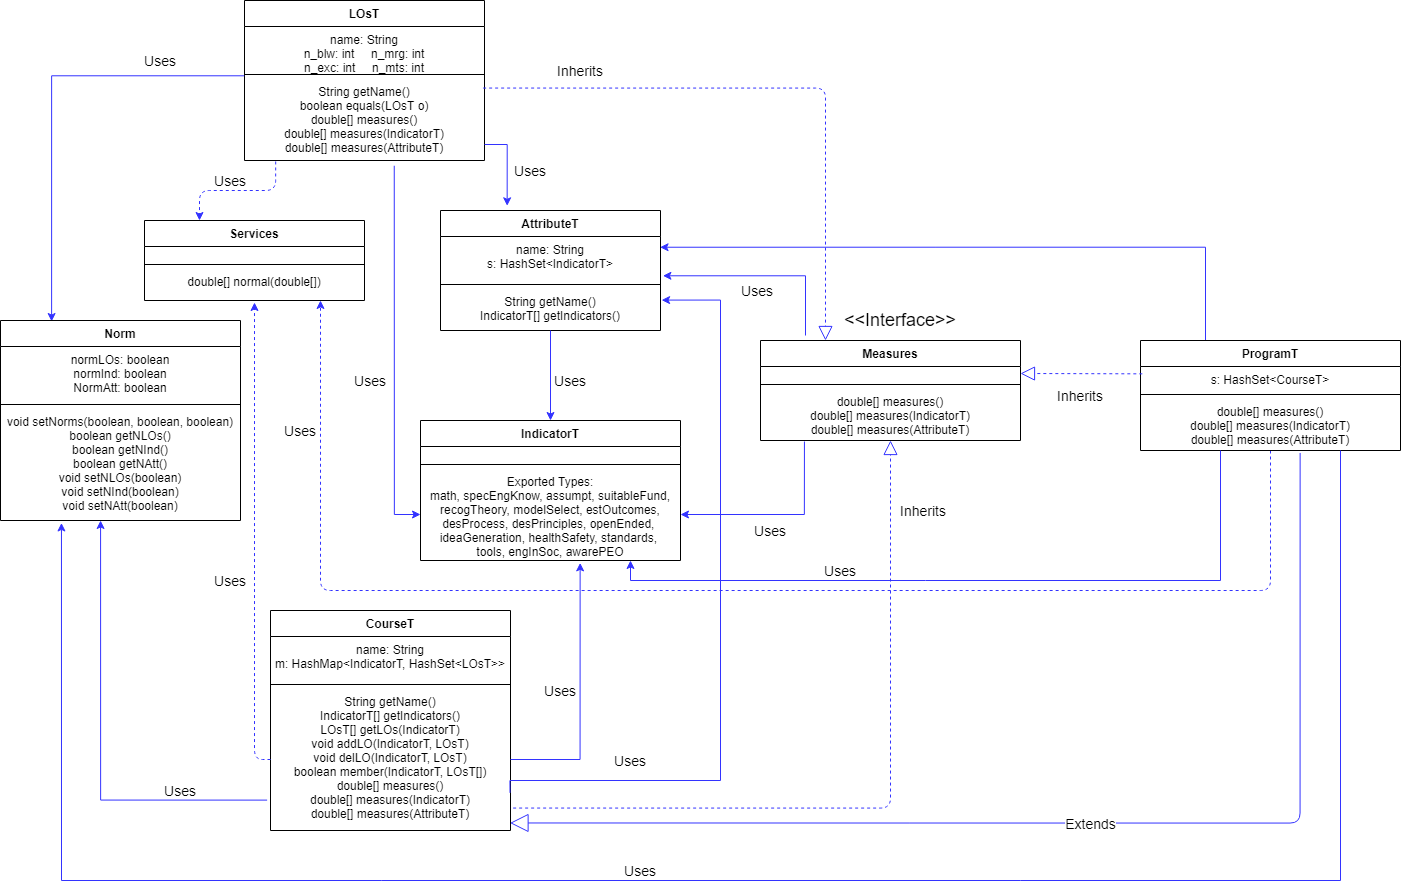
\includegraphics[width=1.2\textwidth]{A3UML.png}
\end{center}

\newpage

\noindent Q2: Draw a control flow graph for the convex hull algorithm.
\begin{center}
  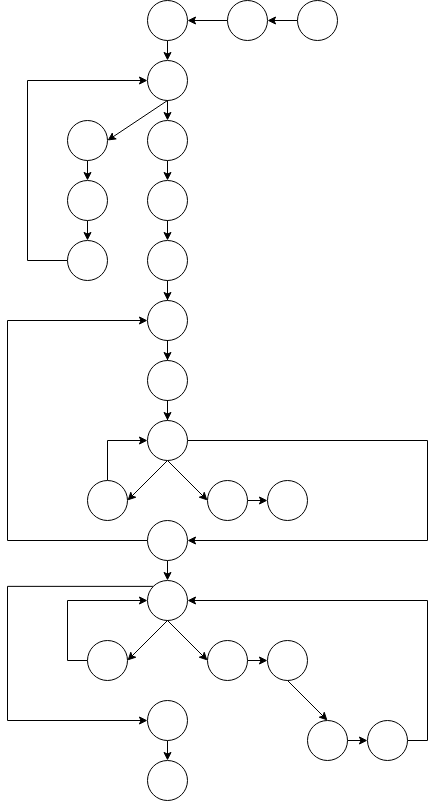
\includegraphics[width=0.5\textwidth]{controlflow.png}
\end{center}


\end {document}


\end{document}